\documentclass[a4paper,10pt]{report}

\def\packagepath{../../../../../preambule}   % path du package principal
\usepackage{\packagepath/preambule}    % utilisation du fichier de configuration

\def\level{BTS }              % Classe
\def\course{CIEL 1}           % Matière
\def\eval{Intégration}          % Titre de l'évaluation

\def\visibleornot{visible}    % visible or invisible
\def\documentpath{./Sources_Latex}
\def\date{C107 - TP3 }
\renewcommand{\arraystretch}{1}  % Ecart dans les tableaux

\def\ptsexoA{0}
\def\ptsexoB{0}

\def\ptstotal{\ptsexoA+\ptsexoB}

\usepackage{hyperref}

\usetikzlibrary{shapes, arrows, positioning}
\usetikzlibrary{shapes.geometric, arrows, positioning, decorations.pathreplacing}

\tikzstyle{etat} = [draw, rounded corners=15pt, minimum width=2.5cm, minimum height=1.2cm, text centered, font=\bfseries]
\tikzstyle{fleche} = [thick, ->, >=stealth]

\usepackage{float}
\usepackage[T1]{fontenc}

% --- L'INTERRUPTEUR ---
\booltrue{afficheCorrige} % Mettez \boolfalse pour masquer le texte (le cadre reste)
%\boolfalse{afficheCorrige} % Mettez \boolfalse pour masquer le texte (le cadre reste)

% --- LA COMMANDE DE CADRE FIXE ---
% #1: Largeur (ex: \linewidth)
% #2: Hauteur (ex: 3cm)
% #3: Contenu de la correction

%\cadreCorrection{width \linewidth}{cm}{}

\begin{document}





\renewcommand{\labelitemi}{\textbullet}

\pagestyle{DS_FP}
\NomPrenomNote{}


\bigskip

\emph{\textbf{Objectif :} Déterminer le paramètre d'un signal amorti à partir de contraintes géométriques, puis valider son étude par la dérivation et l'intégration.}
\medskip

%%=============================================================
\textbf{PARTIE A: Détermination expérimentale du paramètre $c$}


\medskip

On cherche à modéliser un signal par la fonction suivante :  

\[f(x) =  x \e^{-c\cdot x}\] (où $c>0$ est le paramètre à déterminer).
\medskip

Le signal doit respecter la contrainte physique suivante:

\begin{itemize}
    \item le signal doit présenter un maximum à l'instant $x=0,5$ s.
\end{itemize}

\begin{enumerate}
    \item Tracer la courbe de $f$ pour différentes valeurs de $c$.\hfill $\square$
    \item Identifier la valeur de $c$ qui satisfait les contraintes données.\hfill $\square$
    \cadreCorrection{1}{1}{
$c = 2$ satisfait les contraintes, car $f'(0,5) = 0$.
        }
\end{enumerate}

\bigskip

\textbf{PARTIE B: Étude du signal identifié}

\medskip
Utilisez maintenant la valeur trouvée ($c = 2$) pour analyser le comportement du signal $f(x) = x \e^{-2x}$.

\begin{enumerate}
    \item Tracer la courbe de $f$ et observer son comportement.\hfill $\square$
    \item Affichez la fonction dérivée $f'$ \hfill $\square$
    \item Déterminer le signe de $f'$ et en déduire les variations de $f$.\hfill $\square$
    \cadreCorrection{1}{4}{
        \begin{minipage}{0.58\linewidth}
        $f'(x) = \e^{-2x} - 2x \e^{-2x} = \e^{-2x}(1 - 2x)$, qui est positif pour $x < 0,5$ et négatif pour $x > 0,5$.

        Par conséquent, $f$ est strictement croissante sur $[0; 0,5]$ et strictement décroissante sur $[0,5; +\infty[$.
        \end{minipage}\hfill
        \begin{minipage}{0.4\linewidth}
            \begin{tikzpicture}
    \tkzTabInit[lgt=2,espcl=3.5]
    {$x$ / 1, $signe \, f'(x)$ / 1, $var \, f$ / 1}
    {$0$, $+\infty$}
    \tkzTabLine{}
    \tkzTabVar{}
    \end{tikzpicture}
            
        \end{minipage}
    
        }

        
    \item Placer un point $N$ sur la courbe et observer la valeur de $f(N)$ pour différentes positions de $N$. \hfill $\square$
    \item Déplacez le point $N$ vers la droite (grandes valeurs de $x$) et observez la tendance de $f(N)$.\hfill $\square$
    \item Conjecturez la limite de $f(x)$ lorsque $x$ tend vers $+\infty$. \hfill $\square$
    
    \cadreCorrection{1}{3}{
        Lorsque $x$ tend vers $+\infty$, $f(x)$ tend vers 0, car la fonction exponentielle décroît rapidement.

        On peut également calculer la limite formellement :
\[\lim_{x \to +\infty} x \e^{-2x} = \lim_{x \to +\infty} \frac{x}{\e^{2x}}=  0\]



    }

\end{enumerate}

\bigskip

\pagebreak
\thispagestyle{DS_LP}

\textbf{PARTIE C: Intégration et Valeur Moyenne}

\medskip


On souhaite évaluer la tension moyenne délivrée par le composant sur un intervalle $[a ; b]$.


\begin{enumerate}
    \item Créer les curseurs $a$ et $b$ avec les valeurs initiales $a=0$ et $b=2$. \hfill $\square$
    \item Déterminer graphiquement l'aire sous la courbe de $f$ entre $a$ et $b$ avec la commande \verb|Aire = Intégrale(f, a, b)|. \hfill $\square$
    \cadreCorrection{1}{2}{
        D'après Géogébra, l'aire sous la courbe de $f$ entre $a=0$ et $b=2$ est d'environ $0,38$ unités d'aires.
        }
        
    \item Observer comment l'aire change lorsque vous modifiez les valeurs de $a$ et $b$.\hfill $\square$
    \cadreCorrection{1}{3}{
Lorsque vous augmentez $b$, l'aire sous la courbe de $f$ entre $a$ et $b$ augmente, car vous incluez plus de la courbe. Inversement, lorsque vous augmentez $a$, l'aire diminue, car vous excluez une partie de la courbe.

        }

    \item A l'aide de Géogébra, déterminer m'expression d'une primitives $F$ de $f$.\hfill $\square$
    \cadreCorrection{1}{2}{
Une primitive de $f(x) = x \e^{-2x}$ est donnée par :
\[F(x) = -\frac{1}{2}x \e^{-2x} - \frac{1}{4} \e^{-2x} + C\]
        }

    \item Calculer l'aire sous la courbe de $f$ entre $a=0$ et $b=2$ à l'aide de l'intégrale.\hfill $\square$
    \cadreCorrection{1}{3}{
\[\int_0^2 f(x) \, dx = F(2) - F(0) = \left(-\frac{1}{2} \cdot 2 \cdot \e^{-4} - \frac{1}{4} \e^{-4}\right) - \left(-\frac{1}{4}\right) = 0,38\]

L'aire calculée à l'aide de l'intégrale est d'environ $0,38$ unités d'aires, ce qui correspond à l'aire trouvée graphiquement.

        }
    \item Déterminer la valeur moyenne $\mu$ de la fonction $f$ sur l'intervalle $[a ; b]$.\hfill $\square$
    \cadreCorrection{1}{3}{
\[\mu = \frac{1}{b-a} \int_a^b f(x) \, dx = \frac{1}{2-0} \cdot 0,38 = 0,19\]

La valeur moyenne de la fonction $f$ sur l'intervalle $[0 ; 2]$ est d'environ $0,19$ volts.
        }
    \item Créer un rectangle d'équivalence avec les points \verb|(a,0)|, \verb|(b,0)|,\verb|(b, moy)| et \verb|(a, moy)|. 
    
    Utilisez l'outil \verb|Polygone| pour le colorer.\hfill $\square$

    \item En conservant $a=0$, déterminer la valeur de $b$ pour laquelle la valeur moyenne $\mu$ de $f$ sur l'intervalle $[a ; b]$ est égale à $0,1$ volts (à $10^{-2}$ près).\hfill $\square$
    \cadreCorrection{1}{3}{
    A l'aide de Géogébra, on fixera $a=0$ et on fera varier $b$ jusqu'à ce que la valeur moyenne $\mu$ soit égale à $0,1$ volts.

    On obtient une valeur de $b$ d'environ $1,25$.

        }   
\end{enumerate}

         


\end{document}